%!TEX root = main.tex
\section{Checking Synchronizability}\label{sec:verif}

%Verifying synchronizability for a message passing system using a monitor that maintains the conflict-graph of a trace 
%is difficult because it requires dealing with executions where the message buffers are unbounded. 
%For instance, even if the processes are finite-state, this would not lead to a decision procedure. 
We show in this section that checking $k$-synchronizability can be reduced 
to a reachability problem in a system
%~\footnote{Given a system $\mathcal{S}$ and a local state $l$, the reachability problem asks whether $\mathcal{S}$ can reach a configuration that contains the state $l$.} 
that executes under the \emph{$k$-synchronous} semantics 
(where the message buffers cannot grow beyond $k$). The main idea is to show that every
\emph{borderline} synchronizability violation (for which every strict prefix is synchronizable) of a system $\mathcal{S}$ can be ``simulated''
%~\footnote{We refer to the standard notion of (stuttering) simulation where (sequences of) transitions in $\mathcal{S}$ are mapped to transitions of $\mathcal{S'}$.}
by the synchronous semantics of a system $\mathcal{S'}$ where the reception of exactly one message is delayed (w.r.t. the synchronous semantics of $\mathcal{S}$).
Then, we give a monitor which observes executions of $\mathcal{S'}$ and identifies synchronizability violations
(there exists a run of this monitor that goes to an error state whenever such a violation exists). More details and proofs of the results in this section can be found in Appendix~\ref{sec:verif}.

%This result is based on the following ideas:
%\begin{itemize}
%	\item since the set of synchronizable executions is prefix-closed (Lemma~\ref{lem:pref_closed}), it is enough to look for \emph{borderline} violations, i.e., executions which
%are not synchronizable but for which every strict prefix is synchronizable,
%	\item starting from the original system $\mathcal{S}$, define a new system $\mathcal{S'}$ whose synchronous semantics ``simulates'' all the borderline violations of $\mathcal{S}$. 
%	\item define a monitor $\mathcal{M}_{\mathit{causal}}$, which identifies executions of $\mathcal{S'}$ under the synchronous semantics
%which are not executions of the original system $\mathcal{S}$ ($\mathcal{M}_{\mathit{causal}}$ goes to an error state whenever it finds such 
%an execution), 
%	\item define a \emph{monitor} $\mathcal{M}_{\mathit{viol}}$, which identifies synchronizability violations of $\mathcal{S}$ 
%($\mathcal{M}_{\mathit{viol}}$ goes to an error state whenever it finds such an execution),
%	\item establish that $\mathcal{S}$ is $k$-synchronizable whenever the synchronous semantics of $\mathcal{S'}\paral \mathcal{M}_{\mathit{causal}}\paral \mathcal{M}_{\mathit{viol}}$
%doesn't reach a configuration where $\mathcal{M}_{\mathit{viol}}$ is in an error state, but $\mathcal{M}_{\mathit{causal}}$ is \emph{not} in an error state 
%(i.e., reaching such a configuration would mean that the synchronous semantics of $\mathcal{S'}$ admits an execution which is valid according to $\mathcal{S}$ but not synchronizable). 
%\end{itemize}

%\subsection{Synchronizability Violation Patterns}
%
%
%\begin{figure}[t]
%Causal delivery violation:
%\begin{align*}
%\send{1}{p_1,q,\_}\leadsto \send{2}{p_2,q,\_}\mbox{ and }
%\rec{2}{q,\_}  \leadsto_{lossy}  \rec{1}{q,\_} 
%\end{align*}
%Exchange pattern:
%\begin{align*}
%\send{1}{p_1,q_1,\_}\leadsto_{lossy} \rec{2}{q_2,\_}\mbox{ and }
%\send{2}{p_2,q_2,\_}\leadsto_{lossy} \rec{1}{q_1,\_}
%\end{align*}
%\caption{Synchronizability violation patterns.}
%\label{fig:patterns}
%\end{figure}
%
%We show that any trace violating synchronizability contains one of the two violation patterns in Figure~\ref{fig:patterns}.
%Intuitively, the first pattern describes a violation to \emph{causal delivery} where two causally related messages sent to the same process
%are received in an order different from that in which they were sent. Here, the causal order between messages is defined
%by the paths in the action graph (ignoring unmatched sends, the predicate $\leadsto_{lossy}$ is exactly $\leadsto$). 
%The second violation pattern describes a situation in which two messages are sent concurrently 
%and each message is received after the other one is sent. This situation arises for instance in distributed protocols which alternate
%between phases in which all processes send messages to their peers and phases in which they receive messages from their peers. 
%In these cases, the sends and receives in the exchange pattern are causally related since they are executed by the same process.
%
%We say that a trace contains a causal delivery violation or an exchange pattern if it contains the actions and the action-graph paths specified in Figure~\ref{fig:patterns}.
%In the context of matched traces, the predicate $\leadsto_{lossy}$ is exactly $\leadsto$ (describing action-graph paths). Otherwise, the interpretation of $\leadsto_{lossy}$ takes into consideration the fact that the receive action in the right-hand side can occur in the completion of an unmatched trace. 
%Thus, $a \leadsto_{lossy}  \rec{1}{q,\_}$ holds in a trace $t$ when $a$ is an action of $t$ and either $a\leadsto \rec{1}{q,\_}$ (which implies that $\rec{1}{q,\_}$ is also an action of $t$), or $t$ contains an action $b$ such that $\<proc>(b)=q$ and  $a \leadsto b$, or $\<proc>(a)=q$. 
%
%\begin{theorem}\label{th:patt}
%A trace is not synchronizable if{f} it contains a causal delivery violation or an exchange pattern.
%\end{theorem}
%\begin{proof}
%The ``only if'' direction is trivial. For both violation patterns, the two pairs of matching send/receive actions (or one pair and an unmatched send, in the case of the causal delivery violations) will define a conflict graph cycle.
%
%For the ``if'' direction, let $t$ be a non-synchronizable trace. Let us first assume that $t$ is matched. Then, the conflict graph of $t$ contains two nodes $v_1$ and $v_2$ such that there is a path from $v_1$ to $v_2$ and vice-versa. 
%%By an abuse of notation, assume that the action graph contains also edges 
%%$v_1\leadsto v_2$ and $v_2\leadsto v_1$.
%%Let $G_t'$ be the action graph of $t$ extended with edges between every two nodes $u$ and $v$ such that 
%%$\mathrm{act}(u)\in R_{id}$, $\mathrm{act}(v)\in S_{id}$ is an unmatched send, and $\<proc>(\mathrm{act}(u))=\<dest>(\mathrm{act}(v))$.
%%These edges are present in every completion of $t$. By an abuse of notation, for two actions $a$ and $a'$ in $t$, $a\leadsto a'$ (resp., $a\leadsto_1 a'$) denotes the fact that $G'_t$ contains a path (resp., an edge) from the node representing $a$ to that representing $a'$.
%%
%%Let us first assume the case that $G_t'$ is cyclic. By definition, any cycle in $G_t'$ must contain at least one receive action and by Lemma~\ref{lem:acyclic_ag}, at least one of the edges that are not present in $G_t$. Therefore, there exist two actions $\rec{1}{q_1,\_}$ and $\send{2}{p_2,q_1,\_}$, the latter being an unmatched send, such that $\rec{1}{q_1,\_}\leadsto_1 \send{2}{p_2,q_1,\_}$ and $\send{2}{p_2,q_1,\_}\leadsto \rec{1}{q_1,\_}$. 
%%
%%
%%
%%Since we assume well-formed traces, $t$ contains a send action $\send{1}{p_1,q_1,\_}$. Also, since $p_2\neq q_1$, $\send{2}{p_2,q_1,\_}\leadsto \rec{1}{q_1,\_}$ implies that $\send{2}{p_2,q_1,\_}\leadsto \send{1}{p_1,q_1,\_}$.
%%
%%
%%The former implies that there exists a send action $\send{1}{p_1,q_1,\_}$ such that $\send{1}{p_1,q_1,\_}\leadsto \send{2}{p_2,q_1,\_}$ and 
%%
%%TODO THESE PATHS CAN INCLUDE EDGES $\{\send{1}{p_1,q_1,\_},\rec{1}{q_1,\_}\}\rightarrow \{\send{2}{p_3,q_1,\_}\}$ 
%%
%%There are several cases to consider:
%%\begin{itemize}
%Let $\mathrm{act}(v_i)=\{\send{i}{p_i,q_i,\_}, \rec{i}{q_i,\_}\}$, for $i\in [1,2]$. Then, one of the following holds:
%	\begin{itemize}
%		\item $\send{1}{p_1,q_1,\_}\leadsto \send{2}{p_2,q_2,\_}$ and $\rec{2}{q_2,\_}\leadsto \rec{1}{q_1,\_}$, which corresponds to a violation to causal delivery when $q_1=q_2$. Otherwise, when $q_1\neq q_2$, we show that this cycle induces another (smaller cycle) that contains a causal delivery violation. Thus, consider the path between $\rec{2}{q_2,\_}$ and $\rec{1}{q_1,\_}$. By the definition of the conflict relation, the last conflict in this path is necessarily between another action $a$ of $q_1$ (i.e., $\<proc>(a)=q_1$) and $\rec{1}{q_1,\_}$. Otherwise, this path will contain $\send{1}{p_1,q_1,\_}$ and we would have $\send{1}{p_1,q_1,\_}\leadsto  \send{2}{p_2,q_2,\_} \match \rec{2}{q_2,\_}$ and $\rec{2}{q_2,\_}\leadsto \send{1}{p_1,q_1,\_}$ which is impossible by Lemma~\ref{lem:acyclic_ag} (the action graph would be cyclic). Now, the path between $\rec{2}{q_2,\_}$ and $a$ will necessarily contain a conflict due to matching (i.e., a pair of matching send/receive actions); otherwise, $q_1=q_2$. Let $\send{3}{p_3,q_3,\_} \match \rec{3}{q_3,\_}$ be the last such conflict (according to the order in this path). Since it is the last such conflict, we have that $q_3 = q_1$. Therefore, we have $\rec{3}{q_1,\_}\leadsto \rec{1}{q_1,\_}$, and $\send{1}{p_1,q_1,\_}\leadsto \send{2}{p_2,q_2,\_}\match \rec{2}{q_2,\_}\leadsto \send{3}{p_3,q_1,\_}$ which is equivalent to $\send{1}{p_1,q_1,\_}\leadsto \send{3}{p_3,q_1,\_}$. The latter is a violation to causal delivery.
%		
%		\item $\send{1}{p_1,q_1,\_}\leadsto \rec{2}{q_2,\_}$ and $\send{2}{p_2,q_2,\_}\leadsto \rec{1}{q_1,\_}$ which is an exchange pattern.
%		\item $\send{1}{p_1,q_1,\_}\leadsto \rec{2}{q_2,\_}$ and $\rec{2}{q_2,\_}\leadsto \send{1}{p_1,q_1,\_}$ which is impossible by Lemma~\ref{lem:acyclic_ag} because it would imply a cyclic action graph.
%		\item $\rec{1}{q_1,\_}\leadsto \send{2}{p_2,q_2,\_}$ and $\rec{2}{q_2,\_}\leadsto \send{1}{p_1,q_1,\_}$ which is impossible, by Lemma~\ref{lem:acyclic_ag}.
%	\end{itemize}
%%	\item $\mathrm{act}(v_1)=\{\send{1}{p_1,q_1,\_}\}$ and $\mathrm{act}(v_2)=\{\send{2}{p_2,q_2,\_}, \rec{2}{q_2,\_}\}$.
%%\end{itemize}
%%
%%
%%there exist two pairs of matching send/receive actions
%%$\send{1}{p_1,q_1,\_}$, $\rec{1}{q_1,\_}$, and $\send{2}{p_2,q_2,\_}$, $\rec{2}{q_2,\_}$ such that one of the following holds:
%%\begin{itemize}
%%	\item $\send{1}{p_1,q,\_}\leadsto \send{2}{p_2,q,\_}$ and 
%%\end{itemize}
%
%TODO EXTEND TO UNMATCHED TRACES
%\end{proof}

\subsection{Borderline Synchronizability Violations}\label{ssec:verif1}

For a system $\mathcal{S}$, a violation to $k$-synchronizability $e$ is called \emph{borderline} when every strict prefix of 
$e$ is $k$-synchronizable. Figure~\ref{fig:ex-border-sim}(a) gives an example of a borderline violation to $1$-synchronizability (it is the same execution as in Figure~\ref{fig:elevator-exec}(b)).

We show that every borderline violation $e$ ends with a receive action and this action is included in every cycle of $CG_{tr(e)}$ that is 
bad or exceeds the bound $k$. Given a cycle $c = v,v_1,\ldots,v_n,v$ of a conflict graph $CG_t$, the node $v$ is called a \emph{critical} node of $c$ when $(v,v_1)$ is an $SX$ edge with $X\in \{S,R\}$ 
and $(v_n,v)$ is an $YR$ edge with $Y\in \{S,R\}$.


\begin{figure}[t]
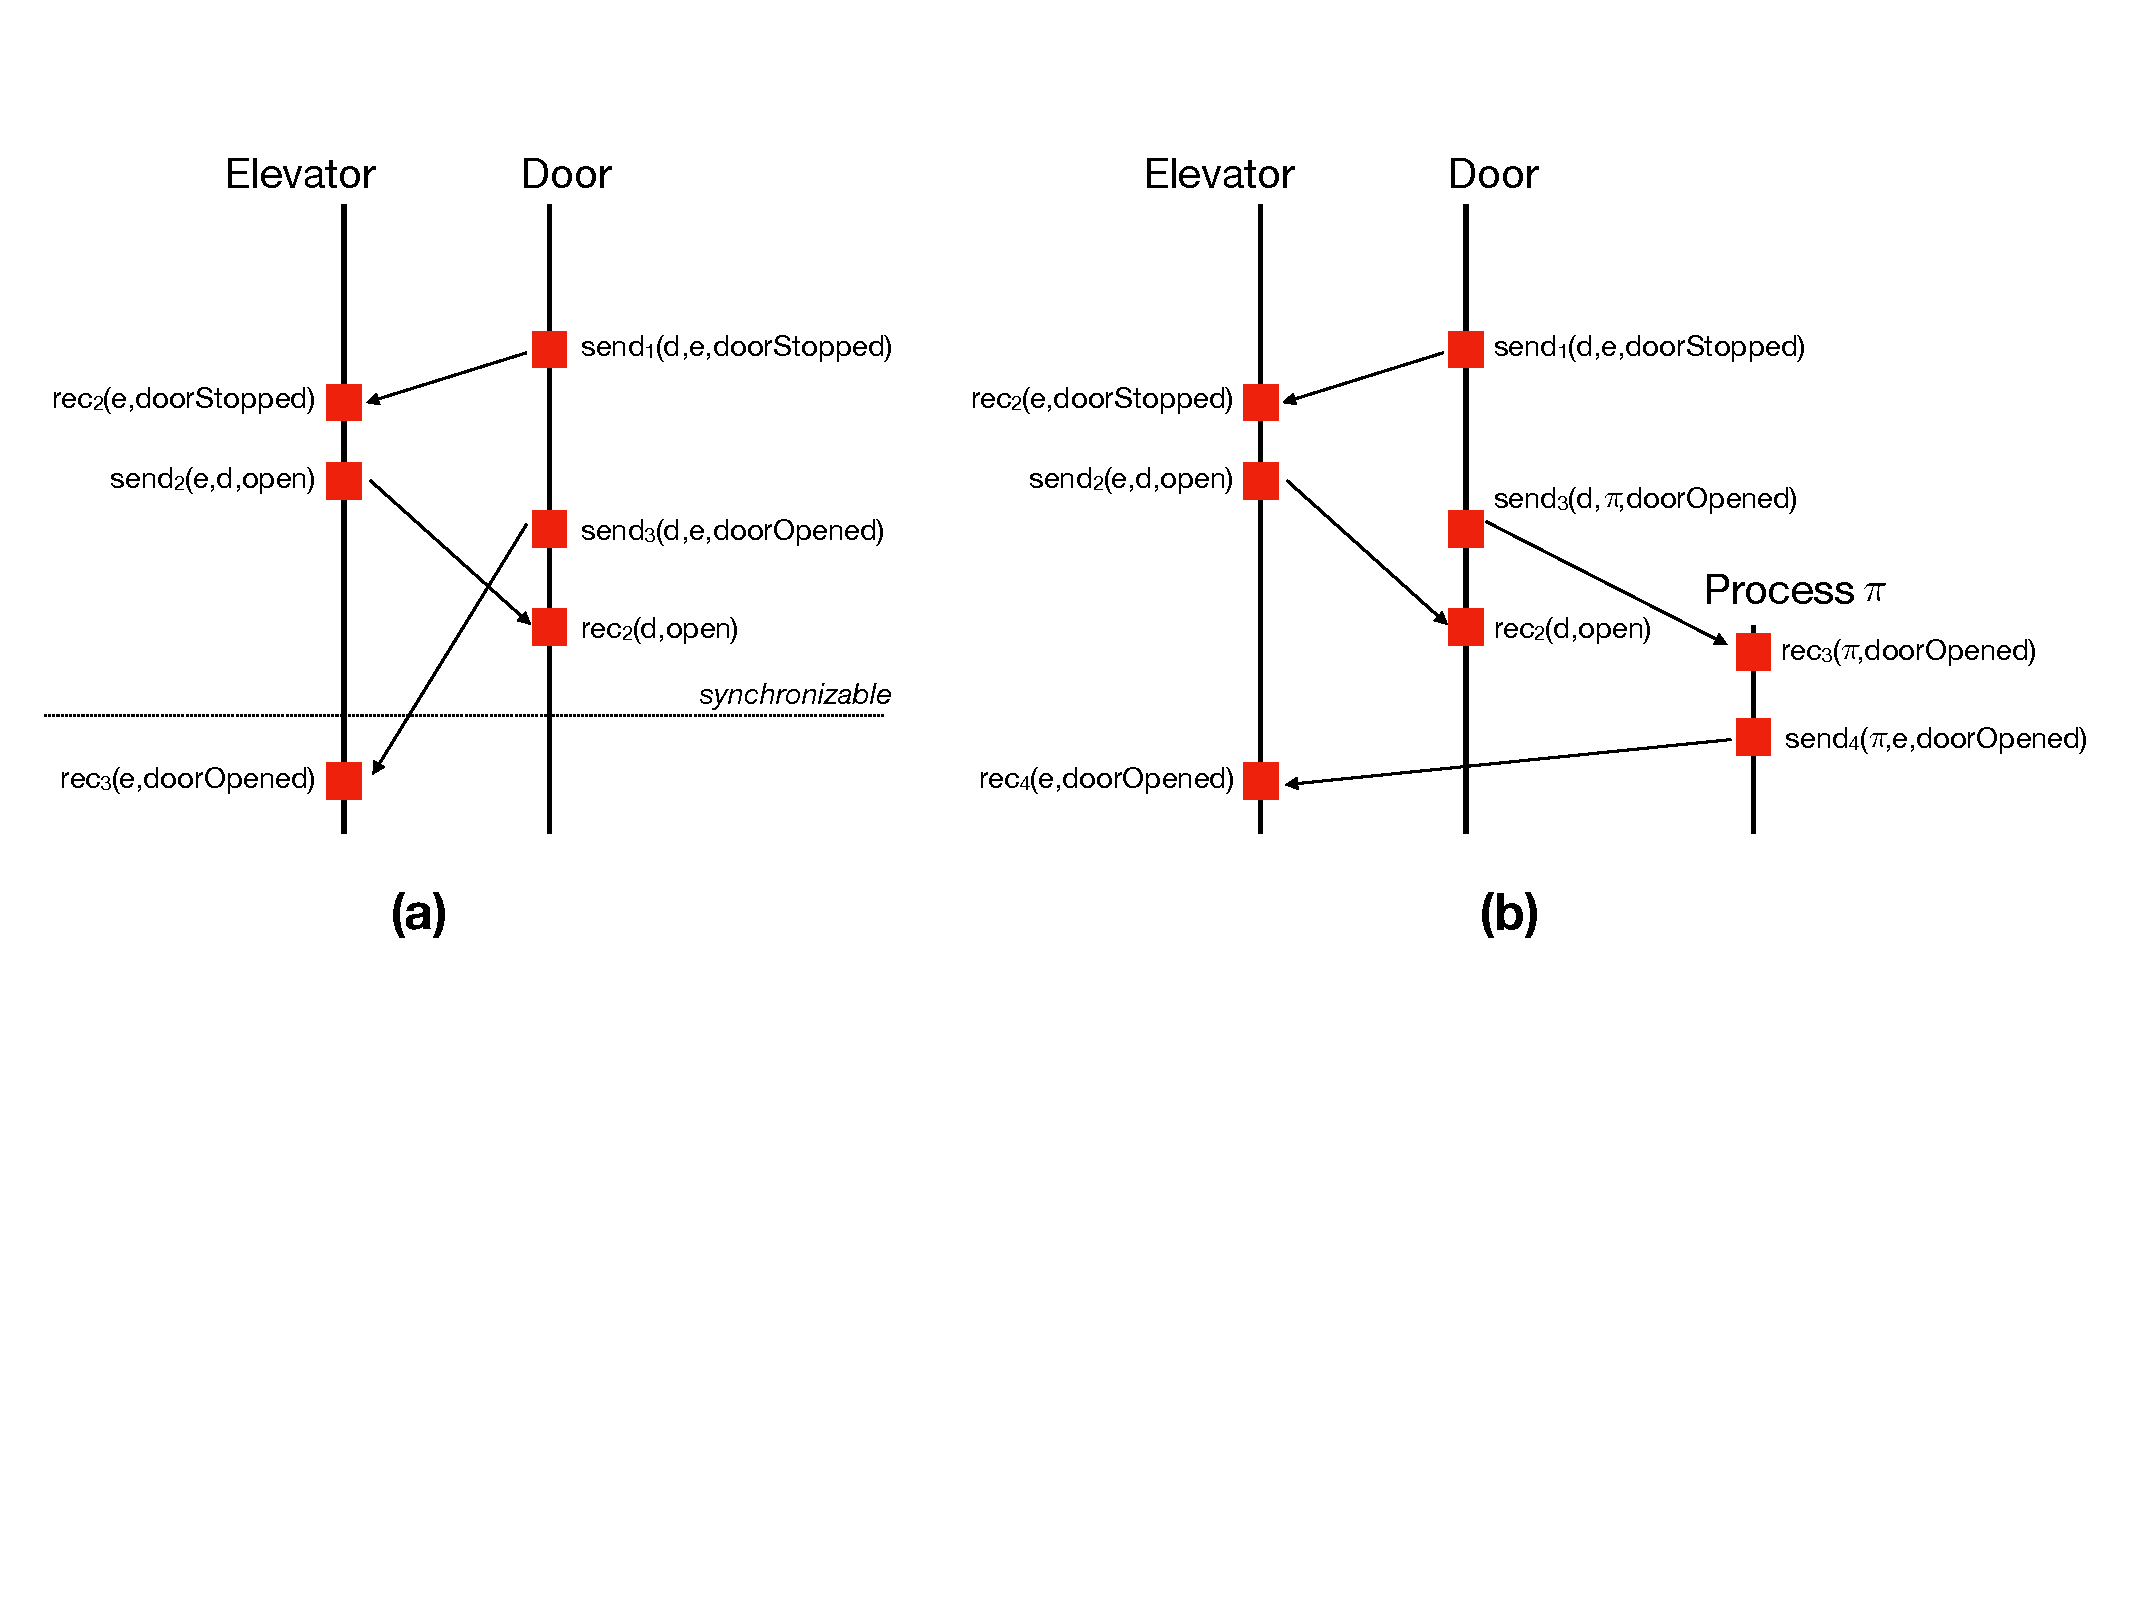
\includegraphics[width=11cm]{Borderline-sim.pdf}
\caption{A borderline violation to $1$-synchronizability.}
\label{fig:ex-border-sim}
\vspace{-5mm}
\end{figure}

\begin{lemma}
Let $e$ be a borderline violation to $k$-synchronizability of $\mathcal{S}$. Then, $e = e'\cdot r$ for some $e'\in (S_{id}\cup R_{id})^*$ and $r\in R_{id}$.
Moreover, the node $v$ of $CG_{tr(e)}$ representing $r$ (and the corresponding send) is a critical node of every cycle of 
$CG_{tr(e)}$ which is bad or of size bigger than $k$. % is of the form $v, v_1,\ldots, v_n,v$ where $(v,v_1)$ is an $SX$ edge for $X\in \{S,R\}$ and $(v_n,v)$ is an $YR$ edge for $Y\in \{S,R\}$.
\end{lemma}


\subsection{Simulating Borderline Violations on the Synchronous Semantics}\label{ssec:verif2}

Let $\mathcal{S'}$ be a system obtained from $\mathcal{S}$ by ``delaying'' the reception of exactly one message, chosen nondeterministically: $\mathcal{S'}$ contains an additional process $\pi$ and exactly one message sent by a process in $\mathcal{S}$ can be non-deterministically redirected to $\pi$ which sends it to the original destination non-deterministically at a later time.
We show that the synchronous semantics of $\mathcal{S'}$ ``simulates'' a permutation of every borderline violation of 
$\mathcal{S}$. 
Figure~\ref{fig:ex-border-sim}(b) shows the synchronous execution of $\mathcal{S'}$ that corresponds to the borderline violation in Figure~\ref{fig:ex-border-sim}(a). It is essentially the same except for delaying the reception of $\text{doorOpened}$ by sending it to $\pi$ who relays it to the elevator at a later time.

%We first show that $\synchExec{\mathcal{S'}}{k}$ contains all the borderline violations of $\mathcal{S}$. 

The following result shows that the $k$-synchronous semantics of $\mathcal{S'}$ ``simulates'' all the borderline violations of $\mathcal{S}$, modulo permutations. 
%For two executions $e$ and $e'$, $e =_{\mathit{id}} e'$ denotes the fact that $e'$ is obtained from $e$ by renaming message identifiers, i.e., there exists a function $f:\<Mids>->\<Mids>$ such that $e[i]=a_j$, for some $a\in S\cup R$ and $j\in\<Mids>$, iff $e'[i]=a_{f(j)}$ (where $e[i]$ denotes the $i$-th element of the sequence $e$).
%TODO BELONGS TO THIS MODULO CONFLICT-PRESERVING PERMUTATIONS
%For a borderline violation $e=e_1\cdot s\cdot e_2\cdot r$, where $s\match r$, we assume that $e_1\cdot s\cdot e_2$ is $k$-synchronous. By Lemma~\ref{lem:zable_nous}, this is without lost of generality because $e_1\cdot s\cdot e_2$ is $k$-synchronizable.

\begin{lemma}
Let $e=e_1\cdot \send{i}{p,q,v}\cdot e_2\cdot \rec{i}{q,v}$ be a borderline violation to $k$-synchronizability of $\mathcal{S}$. Then, $\synchExec{\mathcal{S'}}{k}$ contains an execution $e'$ of the form: 
\begin{align*}
e'=e_1'\cdot \send{i}{p,\pi,(q,v)}\cdot \rec{i}{\pi,(q,v)}\cdot e_2'\cdot \send{j}{\pi,q,v}\cdot \rec{j}{q,v}
\end{align*}
such that $e_1'\cdot \send{i}{p,q,v} \cdot e_2'$ is a permutation of $e_1\cdot \send{i}{p,q,v}\cdot e_2$.
\end{lemma}

%Redirecting messages to $\pi$ may lead to scenarios violating causal delivery (where a message sent later than the redirected one and to the same destination is received earlier). 
%We show how to exclude such scenarios in Section~\ref{ssec:verif3}.
%\subsection{Excluding Executions Violating Causal Delivery}\label{ssec:verif3}
Checking $k$-synchronizability for $\mathcal{S}$ on the system $\mathcal{S'}$ would require that every (synchronous) execution of $\mathcal{S'}$ can be transformed to an execution of $\mathcal{S}$ by applying an homomorphism $\sigma$ where the send/receive pair with destination $\pi$ is replaced with the original send action and the send/receive pair initiated by $\pi$ is replaced with the original receive action (all the other actions are left unchanged). However, this is not true in general. For instance, $\mathcal{S'}$ may admit an execution 
\begin{align*}
\send{i}{p,\pi,(q,v)}\cdot \rec{i}{\pi,(q,v)}\cdot \send{i'}{p,q,v'}\cdot \rec{i'}{q,v'}\cdot \send{j}{\pi,q,v}\cdot \rec{j}{q,v}
\end{align*}
where a message sent after the one redirected to $\pi$ is received earlier (and the two messages were sent by the same process $p$). This execution is possible under the $1$-synchronous semantics of $\mathcal{S'}$. Applying the homomorphism $\sigma$, we get the execution 
$
\send{i}{p,q,v)}\cdot \send{i'}{p,q,v'}\cdot \rec{i'}{q,v'}\rec{i}{q,v}
$
which violates causal delivery and it is thus not possible under the asynchronous semantics of $\mathcal{S}$.
Our solution to this problem is to define a monitor $\mathcal{M}_{\mathit{causal}}$ which excludes such executions of $\mathcal{S'}$ when run under the synchronous semantics, i.e., it goes to an error state whenever applying the homomorphism $\sigma$ leads to a violation of causal delivery. This monitor is based on the same principles that we used to exclude violations of causal delivery in the synchronous semantics in the presence of unmatched sends (the component $B$ from a synchronous configuration). 




\subsection{Detecting Synchronizability Violations}\label{ssec:verif4}

We complete the reduction of checking $k$-synchronizability to a reachability problem under the $k$-synchronous semantics by defining a monitor $\mathcal{M}_{\mathit{viol}}(k)$ which observes executions in $\mathcal{S}_k' \paral\mathcal{M}_{\mathit{causal}}$ and checks whether they represent violations to $k$-synchronizability. We show that there exists a run of $\mathcal{M}_{\mathit{viol}}(k)$ that goes to an error state whenever such a violation exists. 
%The monitor is nondeterministic and it may not reach the error state every time it observes a violation, but there is another run of the monitor on the same execution which reaches the error state. 

Essentially, $\mathcal{M}_{\mathit{viol}}(k)$ observes the sequence of $k$-exchanges in an execution and constructs a conflict graph cycle, interpreting the sequence $\send{i}{p,\pi,(q,v)}\rec{i}{\pi,(q,v)}$ as in the original system $\mathcal{S}$, i.e., as $\send{i}{p,q,v}$, and $\send{i}{\pi,q,v}\rec{i}{q,v}$ as $\rec{i}{q,v}$. 
By Lemma~\ref{lem:critical}, every cycle that is a witness for \emph{non} $k$-synchronizability includes the node representing the pair $\send{i}{p,q,v}$, $\rec{i}{q,v}$. Moreover, the successor of this node in the cycle represents an action that is executed by $p$ and the predecessor an action executed by $q$. Therefore, the monitor searches for a conflict-graph path from a node representing an action of $p$ to a node representing an action of $q$. Whenever it founds such a path it goes to an error state.
The set of executions in $\mathcal{S}_k' \paral\mathcal{M}_{\mathit{causal}}$ for which $\mathcal{M}_{\mathit{viol}}(k)$ goes to an error state %(i.e., the {\tt assert} on the last line of Figure~\ref{fig:mon_viol} fails) 
is denoted by $\mathcal{S}_k' \paral\mathcal{M}_{\mathit{causal}}\paral \neg \mathcal{M}_{\mathit{viol}}(k)$.

\begin{theorem}\label{th:main-verif}
For a given $k$, a system $\mathcal{S}$ is $k$-synchronizable iff 
\begin{align*}
\mathcal{S}_k' \paral\mathcal{M}_{\mathit{causal}}\paral \neg \mathcal{M}_{\mathit{viol}}(k)=\emptyset
\end{align*}
\end{theorem}








